\documentclass[
  coursetitle={Cómputo Nube y Tecnologías Emergentes},
  coursehours={96},
  coursedate={Verano 2026},
  doctype={Práctica},
  otherlangs={english,french},
  authorname={Lázaro},
  authorsurname={Bustio-Martínez},
  authortitle={PhD},
  role={Profesor Investigador},
  email={lbustio@inaoe.mx},
  phone={5559504000},
  ext={7459},
  institution={Instituto Nacional de Astrofísica, Óptica y Electrónica (INAOE)},
  department={Maestría en Ciencias en Tecnologías de Seguridad},
  address={Luis Enrique Erro 1, Sta. Ma. Tonantzintla, San Andrés Cholula, CP 72840, Puebla, México},
  margin={0.5in}
]{../../lbustio_lecture_notes}

\usepackage[utf8]{inputenc}
\usepackage[T1]{fontenc}
\usepackage{array}
\usepackage{tabularx}
\usepackage{enumitem}
\usepackage{longtable}
\usepackage{booktabs}
\usepackage{url}
\usepackage{listings}
\usepackage{xcolor}
\usepackage{graphicx}
\usepackage{tcolorbox}
\usepackage{amssymb}
\usepackage{verbatim}
\usepackage{tikz}
\usetikzlibrary{arrows.meta,backgrounds,fit,positioning}

\definecolor{lightgray}{rgb}{0.97, 0.97, 0.97}
\definecolor{darkblue}{rgb}{0, 0, 0.6}
\definecolor{cloudblue}{HTML}{1F5FA8}
\definecolor{cloudgreen}{HTML}{2E7D59}
\definecolor{cloudorange}{HTML}{B36B00}
\definecolor{cloudred}{HTML}{A83232}
\definecolor{softgray}{HTML}{F5F7FA}

\lstset{
  backgroundcolor=\color{lightgray},
  basicstyle=\ttfamily\small,
  breaklines=true,
  frame=single,
  columns=fullflexible,
  showstringspaces=false,
  commentstyle=\color{gray},
  keywordstyle=\color{darkblue},
  inputencoding=utf8,
  extendedchars=true,
  literate={á}{{\'a}}1 {é}{{\'e}}1 {í}{{\'i}}1 {ó}{{\'o}}1 {ú}{{\'u}}1 {ñ}{{\~n}}1
}

\setlist[itemize]{topsep=0.3em,itemsep=0.2em}
\setlist[enumerate]{topsep=0.3em,itemsep=0.2em}

\tikzset{
  archbox/.style={
    draw=cloudblue,
    fill=cloudblue!7,
    rounded corners=4pt,
    thick,
    align=center,
    text width=3.55cm,
    minimum height=1.05cm,
    inner sep=6pt,
    font=\small
  },
  archboxgreen/.style={
    archbox,
    draw=cloudgreen,
    fill=cloudgreen!8
  },
  archboxorange/.style={
    archbox,
    draw=cloudorange,
    fill=cloudorange!10
  },
  archboxred/.style={
    archbox,
    draw=cloudred,
    fill=cloudred!7
  },
  flowarrow/.style={
    -{Latex[length=3mm,width=2mm]},
    thick,
    draw=darkblue
  }
}

\begin{document}

\IberoCover

%\begin{center}
%    \vspace{0.5cm}
%    \LARGE \textbf{Guía de Laboratorio Operativo y Reproducible} \\
%    \vspace{0.3cm}
%    \huge \textbf{Clase práctica: Detección de ataques de fuerza bruta con ELK}
%    \vspace{0.5cm}
%\end{center}

\section{Propósito de la sesión}

Esta sesión no introduce una práctica completamente nueva. Su propósito es continuar, completar y depurar la actividad de detección de ataques de fuerza bruta con ELK iniciada en la sesión anterior.

Durante la clase, cada estudiante debe terminar de conectar los componentes del pipeline:

\begin{enumerate}
    \item VM en Google Cloud Platform.
    \item Reglas de firewall para acceder a Elasticsearch y Kibana.
    \item Stack ELK ejecutándose con Docker Compose.
    \item Índice de Elasticsearch para almacenar logs.
    \item Agente Python para recolectar logs de \texttt{/var/log}.
    \item Consultas REST para validar datos.
    \item Kibana Discover para explorar eventos.
    \item Dashboard para visualizar intentos fallidos, usuarios e IPs origen.
\end{enumerate}

La meta es que el estudiante pueda explicar cómo un conjunto de logs crudos se transforma en evidencia útil para detectar actividad sospechosa.

\section{Relación con la sesión anterior}

En la sesión anterior se trabajó la actividad de detección de fuerza bruta con ELK. Esa actividad incluía:

\begin{itemize}
    \item abrir puertos en GCP;
    \item levantar Elasticsearch y Kibana;
    \item crear el índice \texttt{gcp-vm-logs};
    \item definir mappings;
    \item ejecutar un script de ingesta en Python;
    \item consultar datos con la API REST;
    \item crear un Data View en Kibana;
    \item analizar eventos de autenticación fallida;
    \item construir visualizaciones.
\end{itemize}

Esta clase práctica está destinada a terminar lo que no haya quedado funcionando, corregir errores y construir el reporte final con evidencias verificables.

\section{Resultado esperado}

Al finalizar la sesión, cada estudiante deberá tener:

\begin{enumerate}
    \item Elasticsearch respondiendo por API REST.
    \item Kibana accesible desde navegador.
    \item El índice \texttt{gcp-vm-logs} creado.
    \item Logs enviados desde la VM hacia Elasticsearch.
    \item Eventos visibles en Kibana Discover.
    \item Al menos una consulta KQL para detectar fallos de autenticación.
    \item Al menos dos visualizaciones en Kibana.
    \item Un dashboard básico de análisis.
    \item Evidencias suficientes para el reporte.
    \item Una reflexión técnica sobre riesgos, costos y límites de la solución.
\end{enumerate}

\section{Regla ética y de seguridad}

\begin{tcolorbox}[title=Uso defensivo y autorizado,colback=cloudred!5,colframe=cloudred]
Esta práctica es defensiva y educativa. Solo se permite analizar logs de la infraestructura propia del estudiante o de recursos autorizados por el profesor.

No se debe intentar generar tráfico, escaneo, autenticaciones fallidas ni pruebas de fuerza bruta contra sistemas de terceros. Si se requiere generar eventos de autenticación fallida para tener datos de prueba, deben generarse únicamente contra la VM propia del estudiante y de forma controlada.
\end{tcolorbox}

\section{Arquitectura de referencia}

La arquitectura mínima esperada es:

\begin{center}
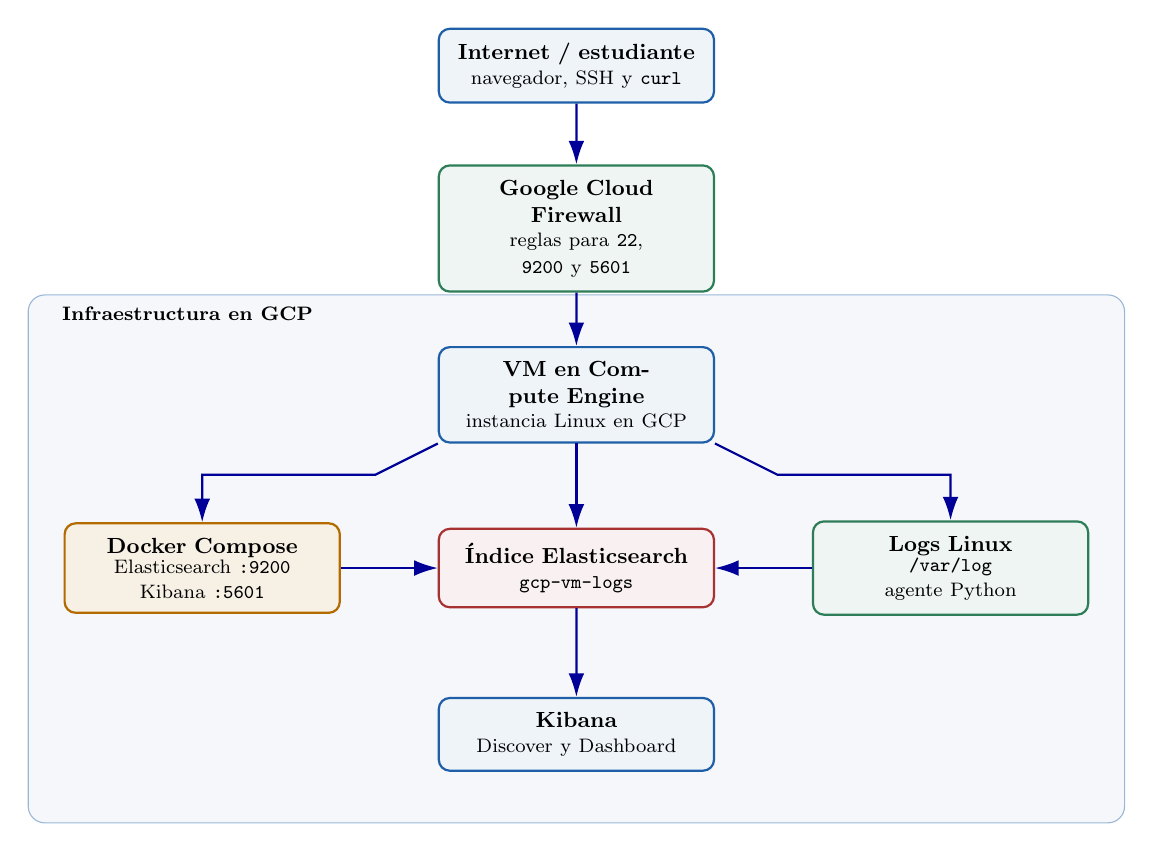
\begin{tikzpicture}[scale=0.88, transform shape]
    \node[archbox] (student) at (0,0) {\textbf{Internet / estudiante}\\[-1pt]\footnotesize navegador, SSH y \texttt{curl}};
    \node[archboxgreen] (firewall) at (0,-2.35) {\textbf{Google Cloud Firewall}\\[-1pt]\footnotesize reglas para \texttt{22}, \texttt{9200} y \texttt{5601}};
    \node[archbox] (vm) at (0,-4.75) {\textbf{VM en Compute Engine}\\[-1pt]\footnotesize instancia Linux en GCP};
    \node[archboxorange] (docker) at (-5.4,-7.25) {\textbf{Docker Compose}\\[-1pt]\footnotesize Elasticsearch \texttt{:9200}\\[-1pt]\footnotesize Kibana \texttt{:5601}};
    \node[archboxred] (index) at (0,-7.25) {\textbf{Índice Elasticsearch}\\[-1pt]\footnotesize \texttt{gcp-vm-logs}};
    \node[archboxgreen] (logs) at (5.4,-7.25) {\textbf{Logs Linux}\\[-1pt]\footnotesize \texttt{/var/log}\\[-1pt]\footnotesize agente Python};
    \node[archbox] (kibana) at (0,-9.65) {\textbf{Kibana}\\[-1pt]\footnotesize Discover y Dashboard};

    \draw[flowarrow] (student) -- (firewall);
    \draw[flowarrow] (firewall) -- (vm);
    \draw[flowarrow] (vm.south west) -- ++(-0.9,-0.45) -| (docker.north);
    \draw[flowarrow] (vm.south) -- (index.north);
    \draw[flowarrow] (vm.south east) -- ++(0.9,-0.45) -| (logs.north);
    \draw[flowarrow] (docker.east) -- (index.west);
    \draw[flowarrow] (logs.west) -- (index.east);
    \draw[flowarrow] (index) -- (kibana);

    \begin{scope}[on background layer]
        \node[
            draw=cloudblue!45,
            fill=softgray,
            rounded corners=6pt,
            inner xsep=0.45cm,
            inner ysep=0.65cm,
            fit=(vm)(docker)(logs)(index)(kibana)
        ] (gcpbox) {};
        \node[
            anchor=west,
            fill=softgray,
            inner xsep=4pt,
            font=\bfseries\footnotesize
        ] at ([xshift=0.35cm,yshift=-0.28cm]gcpbox.north west) {Infraestructura en GCP};
    \end{scope}
\end{tikzpicture}

\small\textbf{Figura:} Flujo mínimo de recolección, ingesta, almacenamiento y análisis de logs.
\end{center}

\section{Puertos utilizados}

\begin{center}
\begin{tabularx}{0.95\textwidth}{|>{\centering\arraybackslash}p{0.14\textwidth}|>{\raggedright\arraybackslash}p{0.25\textwidth}|>{\raggedright\arraybackslash}X|}
\hline
\textbf{Puerto} & \textbf{Servicio} & \textbf{Uso} \\
\hline
22 & SSH & Administración remota de la VM. \\
\hline
9200 & Elasticsearch & API REST e ingesta de documentos. \\
\hline
5601 & Kibana & Interfaz web de análisis. \\
\hline
\end{tabularx}
\end{center}

Los puertos \texttt{9200} y \texttt{5601} deben abrirse solo para la práctica y preferentemente restringirse a la IP pública del estudiante cuando sea posible.

\section{Organización de la clase}

\subsection{Diagnóstico inicial del avance}

Cada estudiante debe comenzar identificando en qué punto se encuentra:

\begin{itemize}
    \item no tengo VM;
    \item tengo VM, pero no tengo Docker;
    \item Docker está instalado, pero ELK no levanta;
    \item Elasticsearch levanta, pero Kibana no responde;
    \item Kibana responde, pero no hay datos;
    \item hay datos, pero no se clasifican eventos de autenticación;
    \item hay datos y necesito construir visualizaciones;
    \item ya tengo dashboard y necesito documentar.
\end{itemize}

El profesor revisará avances a partir de esta lista y priorizará bloqueos.

\subsection{Verificación de la VM}

Entrar por SSH a la VM y ejecutar:

\begin{lstlisting}
hostname
whoami
cat /etc/os-release
free -h
df -h
ip addr
\end{lstlisting}

Estas salidas ayudan a confirmar sistema operativo, usuario, memoria, disco y red.

\subsection{Verificación de firewall en GCP}

Revisar que existan reglas de entrada para los puertos \texttt{9200} y \texttt{5601}, y que apliquen a la VM correcta.

Si se usa etiqueta de red, confirmar que la VM tenga la etiqueta esperada:

\begin{lstlisting}
gcloud compute instances describe NOMBRE_VM --zone ZONA_VM
\end{lstlisting}

Buscar la sección \texttt{tags}.

Ejemplo de reglas de firewall:

\begin{lstlisting}
gcloud compute firewall-rules create allow-kibana-ingress \
  --allow=tcp:5601 \
  --direction=INGRESS \
  --priority=1000 \
  --network=default \
  --target-tags=elk-server

gcloud compute firewall-rules create allow-elasticsearch-rest \
  --allow=tcp:9200 \
  --direction=INGRESS \
  --priority=1000 \
  --network=default \
  --target-tags=elk-server
\end{lstlisting}

Asignar la etiqueta a la VM:

\begin{lstlisting}
gcloud compute instances add-tags NOMBRE_VM \
  --tags=elk-server \
  --zone=ZONA_VM
\end{lstlisting}

Si la regla ya existe, no se debe duplicar. En ese caso se revisa la regla existente.

\subsection{Verificación de Docker y ELK}

Dentro de la VM:

\begin{lstlisting}
docker --version
docker compose version
docker ps
\end{lstlisting}

Si el repositorio \texttt{docker-elk} ya existe:

\begin{lstlisting}
cd ~/docker-elk
docker compose ps
docker compose logs --tail=80 elasticsearch
docker compose logs --tail=80 kibana
\end{lstlisting}

Si el stack no está arriba:

\begin{lstlisting}
cd ~/docker-elk
docker compose up -d
\end{lstlisting}

Validar puertos:

\begin{lstlisting}
ss -tulpn | grep -E "9200|5601"
\end{lstlisting}

Resultado esperado:

\begin{itemize}
    \item Elasticsearch escuchando en \texttt{9200}.
    \item Kibana escuchando en \texttt{5601}.
    \item Contenedores en estado \texttt{Up}.
\end{itemize}

\subsection{Validación de Elasticsearch}

Desde la VM:

\begin{lstlisting}
curl http://localhost:9200/_cluster/health?pretty
\end{lstlisting}

Desde la computadora local, usando la IP pública:

\begin{lstlisting}
curl http://IP_PUBLICA_VM:9200/_cluster/health?pretty
\end{lstlisting}

El estado \texttt{yellow} es aceptable en un laboratorio de un solo nodo. Significa que los shards primarios funcionan, aunque no hay réplicas en otro nodo.

\subsection{Validación de Kibana}

Abrir en el navegador:

\begin{lstlisting}
http://IP_PUBLICA_VM:5601
\end{lstlisting}

Si no abre:

\begin{itemize}
    \item revisar firewall de GCP;
    \item revisar si el contenedor de Kibana está arriba;
    \item revisar logs de Kibana;
    \item confirmar que la URL usa \texttt{http://};
    \item confirmar que la IP pública corresponde a la VM correcta.
\end{itemize}

\section{Creación o revisión del índice}

El índice esperado es:

\begin{lstlisting}
gcp-vm-logs
\end{lstlisting}

Desde Kibana Dev Tools o usando \texttt{curl}, revisar:

\begin{lstlisting}
curl http://localhost:9200/gcp-vm-logs?pretty
\end{lstlisting}

Si el índice no existe, crearlo con un mapping explícito:

\begin{lstlisting}
curl -X PUT "http://localhost:9200/gcp-vm-logs" \
  -H "Content-Type: application/json" \
  -d '{
    "mappings": {
      "properties": {
        "@timestamp": { "type": "date" },
        "log_file": { "type": "keyword" },
        "hostname": { "type": "keyword" },
        "host": { "type": "keyword" },
        "collector_host": { "type": "keyword" },
        "process": { "type": "keyword" },
        "event_type": { "type": "keyword" },
        "username": { "type": "keyword" },
        "source_ip": { "type": "ip" },
        "message": { "type": "text" },
        "raw_line": { "type": "text" },
        "raw_timestamp": { "type": "keyword" }
      }
    }
  }'
\end{lstlisting}

Si el índice ya existe con un mapping incorrecto, se debe documentar el problema antes de borrar. Para reiniciar el índice:

\begin{lstlisting}
curl -X DELETE "http://localhost:9200/gcp-vm-logs"
\end{lstlisting}

Luego se vuelve a crear el índice con el mapping correcto.

\section{Agente Python de ingesta}

La carpeta de la actividad anterior contiene dos archivos de apoyo:

\begin{itemize}
    \item \texttt{setup\_env.sh};
    \item \texttt{collect\_varlog\_to\_elk.py}.
\end{itemize}

El objetivo del agente es leer archivos de \texttt{/var/log}, transformar líneas de log en documentos JSON y enviarlos a Elasticsearch.

\subsection{Preparar entorno Python}

En la VM:

\begin{lstlisting}
sudo apt update
sudo apt install -y python3 python3-venv python3-pip file
\end{lstlisting}

Crear entorno:

\begin{lstlisting}
python3 -m venv elk-logs-env
source elk-logs-env/bin/activate
pip install requests
\end{lstlisting}

Si se usa \texttt{setup\_env.sh}:

\begin{lstlisting}
chmod +x setup_env.sh
./setup_env.sh
source elk-logs-env/bin/activate
\end{lstlisting}

\subsection{Revisar el script antes de ejecutarlo}

Antes de correr el agente, cada estudiante debe revisar:

\begin{itemize}
    \item URL de Elasticsearch;
    \item usuario y contraseña si el stack tiene autenticación;
    \item índice de destino;
    \item límite de líneas por archivo;
    \item exclusión de archivos binarios;
    \item permisos de lectura sobre \texttt{/var/log}.
\end{itemize}

Ejemplo de endpoint si el script corre dentro de la misma VM:

\begin{lstlisting}
ELASTIC_URL = "http://localhost:9200/gcp-vm-logs/_doc"
\end{lstlisting}

Ejemplo de endpoint si el script corre desde otra máquina:

\begin{lstlisting}
ELASTIC_URL = "http://IP_PUBLICA_VM:9200/gcp-vm-logs/_doc"
\end{lstlisting}

No se deben publicar contraseñas ni tokens en el reporte.

\subsection{Ejecutar el agente}

\begin{lstlisting}
source elk-logs-env/bin/activate
python3 collect_varlog_to_elk.py
\end{lstlisting}

Si aparecen errores de permisos en \texttt{/var/log}, se puede ejecutar con \texttt{sudo}, pero documentando la razón:

\begin{lstlisting}
sudo elk-logs-env/bin/python collect_varlog_to_elk.py
\end{lstlisting}

Resultado esperado:

\begin{itemize}
    \item lista de archivos detectados;
    \item mensajes de procesamiento;
    \item conteo final de documentos enviados;
    \item documentos visibles en Elasticsearch.
\end{itemize}

\section{Generación controlada de eventos de autenticación fallida}

Si la VM no tiene suficientes eventos de autenticación fallida, se pueden generar intentos fallidos de forma controlada contra la VM propia.

Desde la computadora del estudiante:

\begin{lstlisting}
ssh usuario_inexistente@IP_PUBLICA_VM
\end{lstlisting}

Ingresar una contraseña incorrecta y cancelar después de pocos intentos.

Reglas:

\begin{itemize}
    \item hacerlo solo contra la VM propia;
    \item no automatizar diccionarios;
    \item no ejecutar ataques contra terceros;
    \item no saturar la VM;
    \item documentar que se generaron eventos controlados de prueba.
\end{itemize}

Después, volver a ejecutar el agente de ingesta para enviar los nuevos logs a Elasticsearch.

\section{Consultas REST de validación}

\subsection{Conteo total de documentos}

\begin{lstlisting}
curl "http://localhost:9200/gcp-vm-logs/_count?pretty"
\end{lstlisting}

\subsection{Buscar eventos relacionados con autenticación fallida}

Si el script clasifica \texttt{event\_type}:

\begin{lstlisting}
curl -X GET "http://localhost:9200/gcp-vm-logs/_search?pretty" \
  -H "Content-Type: application/json" \
  -d '{
    "query": {
      "term": {
        "event_type": "authentication_failure"
      }
    }
  }'
\end{lstlisting}

Si todavía no existe \texttt{event\_type}, buscar en el mensaje:

\begin{lstlisting}
curl -X GET "http://localhost:9200/gcp-vm-logs/_search?pretty" \
  -H "Content-Type: application/json" \
  -d '{
    "query": {
      "match": {
        "message": "Failed password"
      }
    }
  }'
\end{lstlisting}

\subsection{Top de IPs origen}

\begin{lstlisting}
curl -X GET "http://localhost:9200/gcp-vm-logs/_search?pretty" \
  -H "Content-Type: application/json" \
  -d '{
    "size": 0,
    "aggs": {
      "top_source_ip": {
        "terms": {
          "field": "source_ip",
          "size": 10
        }
      }
    }
  }'
\end{lstlisting}

\subsection{Top de usuarios}

\begin{lstlisting}
curl -X GET "http://localhost:9200/gcp-vm-logs/_search?pretty" \
  -H "Content-Type: application/json" \
  -d '{
    "size": 0,
    "aggs": {
      "top_usernames": {
        "terms": {
          "field": "username",
          "size": 10
        }
      }
    }
  }'
\end{lstlisting}

\section{Trabajo en Kibana}

\subsection{Crear Data View}

En Kibana:

\begin{enumerate}
    \item Abrir \texttt{http://IP\_PUBLICA\_VM:5601}.
    \item Ir a \textit{Stack Management}.
    \item Entrar a \textit{Data Views}.
    \item Crear un Data View con el patrón:
\end{enumerate}

\begin{lstlisting}
gcp-vm-logs*
\end{lstlisting}

\begin{enumerate}[resume]
    \item Seleccionar \texttt{@timestamp} como campo de tiempo.
    \item Guardar.
\end{enumerate}

\subsection{Explorar en Discover}

Ir a \textit{Analytics} \(\rightarrow\) \textit{Discover}.

Consultas KQL sugeridas:

\begin{lstlisting}
event_type : "authentication_failure"
\end{lstlisting}

\begin{lstlisting}
message : "Failed password"
\end{lstlisting}

\begin{lstlisting}
message : "Invalid user"
\end{lstlisting}

\begin{lstlisting}
source_ip : *
\end{lstlisting}

\begin{lstlisting}
username : *
\end{lstlisting}

Ajustar el rango temporal a:

\begin{itemize}
    \item Last 15 minutes;
    \item Last 1 hour;
    \item Last 24 hours;
    \item rango personalizado según la hora de la práctica.
\end{itemize}

\subsection{Visualizaciones mínimas}

El dashboard debe incluir al menos:

\begin{enumerate}
    \item Conteo total de eventos.
    \item Conteo de eventos de autenticación fallida.
    \item Top de IPs origen.
    \item Top de usuarios intentados.
    \item Histograma temporal de eventos.
    \item Tabla de eventos recientes con \texttt{@timestamp}, \texttt{source\_ip}, \texttt{username}, \texttt{process} y \texttt{message}.
\end{enumerate}

\section{Guía de troubleshooting}

\subsection{Elasticsearch no responde}

Revisar:

\begin{lstlisting}
docker ps
docker compose logs --tail=80 elasticsearch
curl http://localhost:9200/_cluster/health?pretty
free -h
\end{lstlisting}

Posibles causas:

\begin{itemize}
    \item contenedor caído;
    \item falta de memoria;
    \item puerto no expuesto;
    \item Docker no está ejecutando;
    \item Elasticsearch aún está iniciando.
\end{itemize}

\subsection{Kibana no abre}

Revisar:

\begin{lstlisting}
docker ps
docker compose logs --tail=80 kibana
ss -tulpn | grep 5601
\end{lstlisting}

Posibles causas:

\begin{itemize}
    \item Kibana aún está arrancando;
    \item firewall no permite \texttt{5601};
    \item IP pública incorrecta;
    \item contenedor caído;
    \item Elasticsearch no está listo.
\end{itemize}

\subsection{El agente Python no envía documentos}

Revisar:

\begin{lstlisting}
python3 --version
source elk-logs-env/bin/activate
python3 -c "import requests; print('requests ok')"
curl http://localhost:9200/gcp-vm-logs/_count?pretty
\end{lstlisting}

Posibles causas:

\begin{itemize}
    \item endpoint incorrecto;
    \item autenticación incorrecta;
    \item falta \texttt{requests};
    \item permisos insuficientes para leer \texttt{/var/log};
    \item índice no existe;
    \item mapping incompatible.
\end{itemize}

\subsection{No aparecen eventos de fuerza bruta}

Revisar:

\begin{itemize}
    \item si existen líneas de autenticación fallida en \texttt{/var/log/auth.log};
    \item si el sistema usa otro archivo de logs;
    \item si el parser reconoce los patrones;
    \item si \texttt{event\_type} se está generando correctamente;
    \item si Kibana está filtrando un rango temporal incorrecto.
\end{itemize}

Buscar en la VM:

\begin{lstlisting}
sudo grep -Ei "failed password|invalid user|authentication failure" /var/log/auth.log
\end{lstlisting}

Si no existe \texttt{/var/log/auth.log}, revisar:

\begin{lstlisting}
ls -lah /var/log
journalctl -u ssh --no-pager | tail -50
\end{lstlisting}

\subsection{Error de mapping}

Si Elasticsearch rechaza documentos con \texttt{document\_parsing\_exception}, revisar:

\begin{itemize}
    \item tipo del campo \texttt{source\_ip};
    \item campos enviados por Python;
    \item mapping del índice;
    \item documentos previos que hayan creado mapping dinámico incorrecto.
\end{itemize}

Ver mapping:

\begin{lstlisting}
curl http://localhost:9200/gcp-vm-logs/_mapping?pretty
\end{lstlisting}

\section{Evidencias mínimas para el reporte}

El reporte debe incluir capturas o salidas de terminal de:

\begin{enumerate}
    \item VM activa en GCP.
    \item Reglas de firewall para \texttt{9200} y \texttt{5601}.
    \item Contenedores de ELK ejecutándose.
    \item Respuesta de \texttt{/\_cluster/health}.
    \item Índice \texttt{gcp-vm-logs} creado.
    \item Mapping del índice.
    \item Ejecución del agente Python.
    \item Conteo de documentos en Elasticsearch.
    \item Consulta REST de eventos de autenticación fallida.
    \item Kibana Data View creado.
    \item Discover mostrando eventos.
    \item Consulta KQL usada.
    \item Dashboard con visualizaciones.
    \item Problemas encontrados y soluciones.
    \item Costos observados o estimados.
    \item Medidas de limpieza o cierre de recursos.
\end{enumerate}

\section{Bitácora de trabajo}

Durante la clase, cada estudiante debe mantener una bitácora mínima:

\begin{center}
\begin{tabularx}{0.95\textwidth}{|>{\raggedright\arraybackslash}p{0.12\textwidth}|>{\raggedright\arraybackslash}X|>{\raggedright\arraybackslash}p{0.19\textwidth}|>{\raggedright\arraybackslash}p{0.21\textwidth}|>{\raggedright\arraybackslash}p{0.21\textwidth}|}
\hline
\textbf{Hora} & \textbf{Acción realizada} & \textbf{Resultado} & \textbf{Problema encontrado} & \textbf{Solución aplicada} \\
\hline
 & & & & \\
\hline
 & & & & \\
\hline
 & & & & \\
\hline
\end{tabularx}
\end{center}

Esta bitácora debe alimentar el reporte final.

\section{Preguntas de análisis para el reporte}

Responder:

\begin{enumerate}
    \item ¿Qué diferencia hay entre logs crudos y eventos estructurados?
    \item ¿Por qué es útil transformar logs en documentos JSON?
    \item ¿Qué función cumple Elasticsearch en esta práctica?
    \item ¿Qué función cumple Kibana?
    \item ¿Qué evidencia permite afirmar que hubo intentos de autenticación fallida?
    \item ¿Qué usuario fue intentado con mayor frecuencia?
    \item ¿Qué IP origen generó más eventos sospechosos?
    \item ¿El patrón parece ataque dirigido o escaneo automatizado? Justificar.
    \item ¿Qué limitaciones tiene el parser usado?
    \item ¿Qué riesgos implica exponer SSH, Elasticsearch y Kibana a Internet?
    \item ¿Qué regla de firewall o medida de hardening propondrías para reducir riesgo?
    \item ¿Qué costos o consumo de recursos observaste en la VM?
\end{enumerate}

\section{Estructura sugerida del reporte}

El PDF debe seguir esta estructura:

\begin{enumerate}
    \item Portada.
    \item Objetivo de la práctica.
    \item Arquitectura implementada.
    \item Configuración de GCP y firewall.
    \item Despliegue de ELK.
    \item Creación del índice y mapping.
    \item Agente Python de ingesta.
    \item Consultas REST de validación.
    \item Exploración en Kibana Discover.
    \item Dashboard creado.
    \item Análisis de eventos de fuerza bruta.
    \item Problemas encontrados y soluciones.
    \item Riesgos y recomendaciones de seguridad.
    \item Costos observados.
    \item Conclusiones.
    \item Evidencias.
\end{enumerate}

\section{Criterios de evaluación}

\begin{center}
\begin{tabularx}{0.75\textwidth}{|>{\raggedright\arraybackslash}X|>{\centering\arraybackslash}p{0.22\textwidth}|}
\hline
\textbf{Criterio} & \textbf{Ponderación} \\
\hline
Stack ELK funcional & 20\% \\
\hline
Ingesta correcta de logs & 20\% \\
\hline
Consultas REST y validación de datos & 15\% \\
\hline
Uso de Kibana Discover y Dashboard & 20\% \\
\hline
Análisis de fuerza bruta & 15\% \\
\hline
Reporte, evidencias y reflexión técnica & 10\% \\
\hline
\end{tabularx}
\end{center}

\section{Cierre de la sesión}

Antes de terminar, cada estudiante debe confirmar:

\begin{itemize}
    \item que tiene capturas suficientes;
    \item que el índice contiene documentos;
    \item que puede consultar eventos en Discover;
    \item que guardó o documentó su dashboard;
    \item que anotó problemas y soluciones;
    \item que no publicó credenciales;
    \item que revisó costos;
    \item que apagó o protegió recursos si ya no los usará.
\end{itemize}

La práctica se considera completa cuando el estudiante puede demostrar el flujo completo: logs de Linux, ingesta con Python, almacenamiento en Elasticsearch, consulta REST, exploración en Kibana y análisis razonado de intentos de fuerza bruta.

\end{document}
